\documentclass[12pt,a4paper]{article}


\usepackage[in, plain]{fullpage}
\usepackage{array}
\usepackage{../../../pas-math}
\usepackage{../../../moncours}



%-------------------------------------------------------------------------------
%          -Packages nécessaires pour écrire en Français et en UTF8-
%-------------------------------------------------------------------------------
\usepackage[utf8]{inputenc}
\usepackage[frenchb]{babel}
\usepackage[T1]{fontenc}
\usepackage{lmodern}
\usepackage{textcomp}



%-------------------------------------------------------------------------------

%-------------------------------------------------------------------------------
%                          -Outils de mise en forme-
%-------------------------------------------------------------------------------
\usepackage{hyperref}
\hypersetup{pdfstartview=XYZ}
%\usepackage{enumerate}
\usepackage{graphicx}
\usepackage{multicol}
\usepackage{tabularx}
\usepackage{multirow}


\usepackage{anysize} %%pour pouvoir mettre les marges qu'on veut
%\marginsize{2.5cm}{2.5cm}{2.5cm}{2.5cm}

\usepackage{indentfirst} %%pour que les premier paragraphes soient aussi indentés
\usepackage{verbatim}
\usepackage{enumitem}
\usepackage[usenames,dvipsnames,svgnames,table]{xcolor}

\usepackage{variations}

%-------------------------------------------------------------------------------


%-------------------------------------------------------------------------------
%                  -Nécessaires pour écrire des mathématiques-
%-------------------------------------------------------------------------------
\usepackage{amsfonts}
\usepackage{amssymb}
\usepackage{amsmath}
\usepackage{amsthm}
\usepackage{tikz}
\usepackage{xlop}
%-------------------------------------------------------------------------------



%-------------------------------------------------------------------------------


%-------------------------------------------------------------------------------
%                    - Mise en forme avancée
%-------------------------------------------------------------------------------

\usepackage{ifthen}
\usepackage{ifmtarg}


\newcommand{\ifTrue}[2]{\ifthenelse{\equal{#1}{true}}{#2}{$\qquad \qquad$}}

%-------------------------------------------------------------------------------

%-------------------------------------------------------------------------------
%                     -Mise en forme d'exercices-
%-------------------------------------------------------------------------------
%\newtheoremstyle{exostyle}
%{\topsep}% espace avant
%{\topsep}% espace apres
%{}% Police utilisee par le style de thm
%{}% Indentation (vide = aucune, \parindent = indentation paragraphe)
%{\bfseries}% Police du titre de thm
%{.}% Signe de ponctuation apres le titre du thm
%{ }% Espace apres le titre du thm (\newline = linebreak)
%{\thmname{#1}\thmnumber{ #2}\thmnote{. \normalfont{\textit{#3}}}}% composants du titre du thm : \thmname = nom du thm, \thmnumber = numéro du thm, \thmnote = sous-titre du thm

%\theoremstyle{exostyle}
%\newtheorem{exercice}{Exercice}
%
%\newenvironment{questions}{
%\begin{enumerate}[\hspace{12pt}\bfseries\itshape a.]}{\end{enumerate}
%} %mettre un 1 à la place du a si on veut des numéros au lieu de lettres pour les questions 
%-------------------------------------------------------------------------------

%-------------------------------------------------------------------------------
%                    - Mise en forme de tableaux -
%-------------------------------------------------------------------------------

\renewcommand{\arraystretch}{1.7}

\setlength{\tabcolsep}{1.2cm}

%-------------------------------------------------------------------------------



%-------------------------------------------------------------------------------
%                    - Racourcis d'écriture -
%-------------------------------------------------------------------------------

% Angles orientés (couples de vecteurs)
\newcommand{\aopp}[2]{(\vec{#1}, \vec{#2})} %Les deuc vecteurs sont positifs
\newcommand{\aopn}[2]{(\vec{#1}, -\vec{#2})} %Le second vecteur est négatif
\newcommand{\aonp}[2]{(-\vec{#1}, \vec{#2})} %Le premier vecteur est négatif
\newcommand{\aonn}[2]{(-\vec{#1}, -\vec{#2})} %Les deux vecteurs sont négatifs

%Ensembles mathématiques
\newcommand{\naturels}{\mathbb{N}} %Nombres naturels
\newcommand{\relatifs}{\mathbb{Z}} %Nombres relatifs
\newcommand{\rationnels}{\mathbb{Q}} %Nombres rationnels
\newcommand{\reels}{\mathbb{R}} %Nombres réels
\newcommand{\complexes}{\mathbb{C}} %Nombres complexes


%Intégration des parenthèses aux cosinus
\newcommand{\cosP}[1]{\cos\left(#1\right)}
\newcommand{\sinP}[1]{\sin\left(#1\right)}


%Probas stats
\newcommand{\stat}{statistique}
\newcommand{\stats}{statistiques}
%-------------------------------------------------------------------------------

%-------------------------------------------------------------------------------
%                    - Mise en page -
%-------------------------------------------------------------------------------

\newcommand{\twoCol}[1]{\begin{multicols}{2}#1\end{multicols}}


\setenumerate[1]{font=\bfseries,label=\textit{\alph*})}
\setenumerate[2]{font=\bfseries,label=\arabic*)}


%-------------------------------------------------------------------------------
%                    - Elements cours -
%-------------------------------------------------------------------------------







\date{}
\title{}

\begin{document}



\begin{tikzpicture}[node distance=2cm]

\node (start) [startstop] {D\'ebut};
\node (pr1) [process, below of=start] {Caluler le discriminant  $\Delta = b^2-4ac$};
\node (dec1) [decision, below of=pr1, yshift=-0.5cm] {$\Delta = 0 ?$};
\node (dec2) [decision, below of=dec1, yshift=-1cm] {$\Delta > 0 ?$};
\node (pr3) [process, below of=dec2, yshift=-0.5cm] {2 solutions $\dfrac{-b +/- \sqrt{\Delta}}{2a}$};
\node (pr2) [process, left of=pr3, xshift=-2cm] {1 solution $\dfrac{-b}{2a}$ };
\node (pr4) [process, right of=pr3, xshift= 2cm] {Aucune solution };
\node (stop) [startstop, below of=pr3] {Fin};


\draw [arrow] (start) --  (pr1);
\draw [arrow] (pr1) --  (dec1);
\draw [arrow] (dec1) -| node[anchor=east] {oui} (pr2);
\draw [arrow] (dec1) -- node[anchor=east] {non} (dec2);
\draw [arrow] (dec2) -- node[anchor=east] {oui} (pr3);
\draw [arrow] (dec2) -| node[anchor=west] {non} (pr4);
\draw [arrow] (pr2) |-  (stop);
\draw [arrow] (pr3) --  (stop);
\draw [arrow] (pr4) |-  (stop);
\end{tikzpicture}



\newpage

\begin{tabular}{cc }
	\begin{footnotesize}
	\begin{tikzpicture}%[scale=0.7]
		\tkzTabInit[lgt=3]
		{$x$                                  /1,
		Signe de\\ $ax^2+bx+c$                    /1.5
		}
		%
		{$-\infty$,$+\infty$}
		%
		\tkzTabLine { ,+, }
	\end{tikzpicture}
\end{footnotesize}
 &
	
	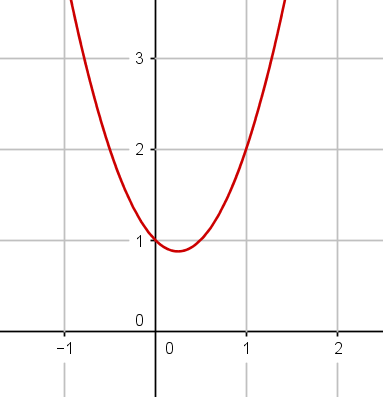
\includegraphics[scale=0.3]{./img/fig_5}\\
\end{tabular}



\begin{tabular}{cc }
	\begin{tabular}{|@{\ }l@{\ }|@{\ }c@{\ }|@{\ }c@{\ }|@{$\qquad$ }c@{$\qquad$ }|}
	\hline
                       & Nombre de      & Nombre de         &       \\
                       & familles ayant & familles n'ayant  & Total \\
                       & un téléviseur  & pas de téléviseur &       \\ \hline
Nombre de familles     & \num{2450}     &   \num{550}       &   \num{300}    \\
ayant une voiture      &                &                   &       \\ \hline
Nombre de familles     &  \num{800}     &   \num{1200}      &   \num{2000}    \\
n'ayant pas de voiture &                &                   &       \\ \hline
Total                  &  \num{3250}    &   \num{1750}      & 5000  \\ \hline
\end{tabular} &
	
	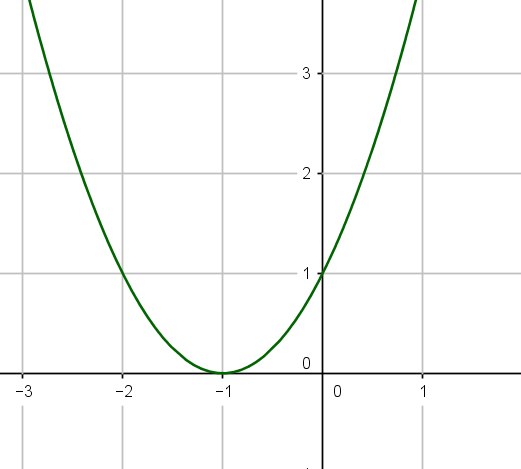
\includegraphics[scale=0.25]{./img/fig_1}\\
\end{tabular}	



\begin{tabular}{cc }
	\begin{footnotesize}
	\begin{tikzpicture}[scale=0.7]
		\tkzTabInit[lgt=3]
		{$x$                                  /1,
			Signe de\\ $ax^2+bx+c$                    /1.5
		}
		%
		{$-\infty$,$x_1$, $x_2$,$+\infty$}
		%
		\tkzTabLine { ,+,z, -, z,+, }
	\end{tikzpicture}
\end{footnotesize}
 &
	
	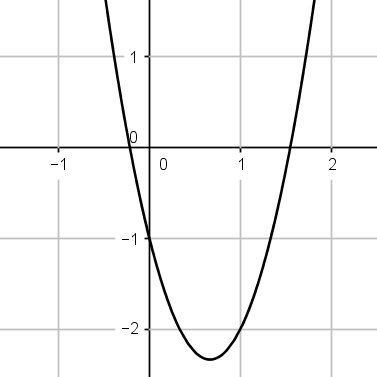
\includegraphics[scale=0.25]{./img/fig_3}\\
\end{tabular}


\begin{tabular}{cc }
	\begin{footnotesize}
	\begin{tikzpicture}%[scale=0.7]
		\tkzTabInit[lgt=3]
		{$x$                                  /1,
		Signe de\\ $ax^2+bx+c$                    /1.5
		}
		%
		{$-\infty$,$+\infty$}
		%
		\tkzTabLine { ,-, }
	\end{tikzpicture}
\end{footnotesize}
 &
	
	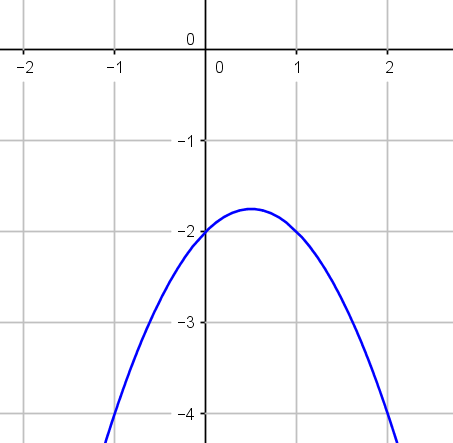
\includegraphics[scale=0.25]{./img/fig_6}\\
\end{tabular}


\begin{tabular}{cc }
	\begin{scriptsize}
\begin{tikzpicture}[scale=0.6]
\tkzTabInit[lgt=3]
{$x$                                  /1,
	Signe de\\ $ax^2+bx+c$                    /2.5
 }
%
{$-\infty$,$x_1$,$+\infty$}
%
\tkzTabLine { ,-,z,-, }
	\end{tikzpicture}
\end{scriptsize}
 &
	
	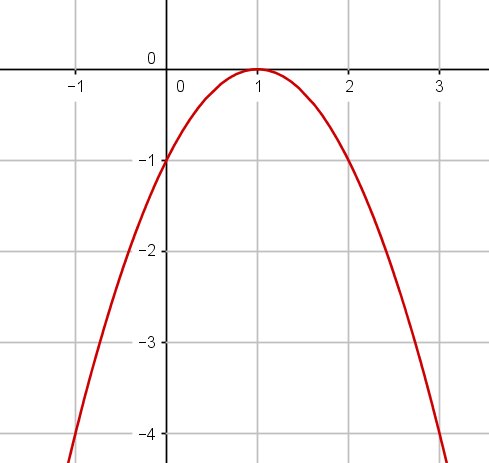
\includegraphics[scale=0.25]{./img/fig_2}\\
\end{tabular}



\begin{tabular}{ll }
	\begin{scriptsize}
	\begin{tikzpicture}[scale=0.6]
		\tkzTabInit[lgt=3]
		{$x$                                  /1,
			Signe de\\ $ax^2+bx+c$\\ (si $x_1 < x_2$)                    /2.5
		}
		%
		{$-\infty$,$x_1$, $x_2$,$+\infty$}
		%
		\tkzTabLine { ,-,z, +, z,-, }
	\end{tikzpicture}
\end{scriptsize}
 &
	
	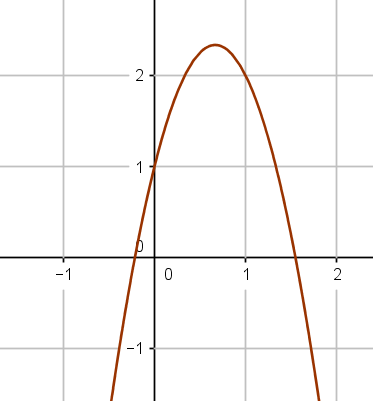
\includegraphics[scale=0.25]{./img/fig_4}\\
\end{tabular}
	


%

\begin{tikzpicture}[node distance=2cm]

\node (start) [startstop] {D\'ebut};
\node (pr1) [process, below of=start] {Caluler le discriminant  $\Delta = b^2-4ac$};
\node (dec1) [decision, below of=pr1, yshift=-0.5cm] {$\Delta = 0 ?$};
\node (dec2) [decision, below of=dec1, yshift=-1cm] {$\Delta > 0 ?$};
\node (pr3) [process, below of=dec2, yshift=-0.5cm] {2 solutions $\dfrac{-b +/- \sqrt{\Delta}}{2a}$};
\node (pr2) [process, left of=pr3, xshift=-2cm] {1 solution $\dfrac{-b}{2a}$ };
\node (pr4) [process, right of=pr3, xshift= 2cm] {Aucune solution };
\node (stop) [startstop, below of=pr3] {Fin};


\draw [arrow] (start) --  (pr1);
\draw [arrow] (pr1) --  (dec1);
\draw [arrow] (dec1) -| node[anchor=east] {oui} (pr2);
\draw [arrow] (dec1) -- node[anchor=east] {non} (dec2);
\draw [arrow] (dec2) -- node[anchor=east] {oui} (pr3);
\draw [arrow] (dec2) -| node[anchor=west] {non} (pr4);
\draw [arrow] (pr2) |-  (stop);
\draw [arrow] (pr3) --  (stop);
\draw [arrow] (pr4) |-  (stop);
\end{tikzpicture}


	
\end{document}